\documentclass[a4paper]{article}
\usepackage{amssymb, amsmath}
\usepackage{graphicx}
\begin{document}
\section{Linear Regression}
\subsection{Linear regression and Least Square Solution}
\begin{align*}
Y = X{\boldsymbol \beta} + \epsilon
\end{align*}
Where Y is a n $\times$ 1 matrix, X is a n $\times$ k matrix, beta is k $\times$ 1 vector and $\epsilon$ is nx1 vector with $\epsilon_i$ begin iid with normal distribution.\\
{\bf Assumptions}\\
1. Linear \\
2. X matrix has full rank. In other words, no multicollinearity. \\
2. error term has zero mean $E[\epsilon|X] = 0$\\
3. Homescedasticity or equal variance of $\epsilon$. In other words, no autocorrelation between disturbances.$cov(\epsilon_i, \epsilon_j)=0$.\\
6. Number of obsearvations n must be greater than the number of parameters.\\
{\bf Least Square Solution}\\
The cost function is given by
\begin{align*}
f(\boldsymbol \beta) = ||Y-X\beta||^2 & = (Y-X\beta)^T(Y-X\beta)
                      & = Y^T Y - Y^TX\beta - \beta^TX^TY +\beta^TX^T X \beta
\end{align*}
Since third term are scalar, 
\begin{align*}
 \beta^TX^TY = (\beta^TX^TY)^T = Y^TX\beta 
\end{align*}
\begin{align*}
f(\beta) = Y^T Y - 2Y^TX\beta - \beta^TX^T X \beta
            = Y^T Y - 2(X^TY)^T\beta + \beta^TX^T X \beta
\end{align*}
The first term is a constant and its derivative is zero. \\
{\bf The deriviative of 2nd term}\\
Consider the derivative of $\alpha^T \beta$ with respect to $\beta$.
\begin{align*}
\boldsymbol{\alpha}^T \boldsymbol{\beta} = \Sigma \alpha_i \beta_i \\
\frac{\partial{\boldsymbol{\alpha}^T\boldsymbol{\beta}}}{\partial \beta_i} = \alpha_i\\
\end{align*}
Write the derivative in matrix form
\begin{align*}
\left(  \begin{array} {c}
		\frac{\partial{\boldsymbol{\alpha}^T\boldsymbol{\beta}}}{\partial \beta_1}\\
		\frac{\partial{\boldsymbol{\alpha}^T \boldsymbol{\beta}}}{\partial \beta_2}\\
                  ...\\
		\frac{\partial{\boldsymbol{\alpha}^T \boldsymbol{\beta}}}{\partial \beta_3}\\
		\end{array}
		\right) 
=\left(  \begin{array} {c}
		\alpha_1\\
		\alpha_2\\
                  ...\\
		\alpha_p\\
		\end{array}
		\right) 
\end{align*}
So if we let $\alpha= X^TY$, we have
\begin{align*}
\frac{\partial{2(X^TY)^T\beta}}{\partial \beta} = 2X^TY
\end{align*}
{\bf The derivative of 3rd term}\\
let $A=X^TX$,
\begin{align*}
\beta^TX^T X \beta = \beta^T
\left(  \begin{array} {c}
		\Sigma_i A_{1k}\beta_{k}\\
		 \Sigma_i A_{2k}\beta_{k}\\
                  ...\\
		 \Sigma_k A_{pk}\beta_{k}\\
		\end{array}
		\right) 
 =  \Sigma_j \beta_j (\Sigma_k A_{jk}\beta_k)
\end{align*}
To calculate the derivative of $f(\beta)$, we note there are only 3 cases that the derivative does not vanish\\
1) l = j = k 
\begin{align*}
\frac{f(\boldsymbol \beta)}{\partial \beta_l} 
= 2 A_{ll} \beta_l 
\end{align*}
2) l=j, j $\neq$ k
\begin{align*}
\frac{f(\boldsymbol \beta)}{\partial \beta_l} 
= \Sigma_{k, k\neq l} A_{lk}\beta_{k}\\
\end{align*}
3) l=k, j $\neq$ k
\begin{align*}
\frac{f(\boldsymbol \beta)}{\partial \beta_l} 
= \Sigma_{j, j\neq l} A_{jl}\beta_{j} = \Sigma_{j,  j\neq l} A^T_{lj}\beta{j}
\end{align*}
Therefore
\begin{align*}
\frac{f(\boldsymbol \beta)}{\partial \beta_l}  = A_{ll} \beta_l + \Sigma_{k, k\neq l} A_{lk}\beta_{k} + A_{ll} \beta_l + \Sigma_{j, j \neq l} A^T_{lj}\beta{j} \\
= \Sigma_{k} A_{lk}\beta_{k} + \Sigma_{j} A^T_{lj}\beta{j}
\end{align*}
The first term is the lth row of vector $A\beta = X^TX\beta$, and the 2nd term is the lth row of vector$A^T\beta=X^TX\beta$. So we put the whole derivative in matrix form
\begin{align*}
\frac{f(\boldsymbol \beta)}{\partial {\boldsymbol \beta}} = -2X^TY+2X^TX\beta
\end{align*}
which is a px1 vector with each row corresponding to the derivative with respect to $\beta_i$
letting the derivative equal to zero yields the {\bf normal equation} and the estimation of $\beta$\\
Normal equation
\begin{align*}
(X^TX) \hat \beta = X^TY
\end{align*}
Estimator of $\beta$
\begin{align*}
\hat \beta = (X^TX)^{-1}X^TY
\end{align*}
{\bf Least Square Estimator for Simple Linear Regression}\\
\begin{align*}
y =  \beta_o + \beta_1 X + \epsilon\\
\end{align*}
\begin{align*}
	&\left(  \begin{array} {c}
		\beta_{0} \\
		\beta_{1} \\
		\end{array}
		\right) \\
=& (X^TX)^{-1}X^TY \\
=&\left( \left(  \begin{array} {cccc}
		1 & 1 &... &1\\
		x_1 & x_2 &... &x_n \\
		\end{array}
		\right) 
    \left(  \begin{array} {cc}
		1 & x_1 \\
		1 & x_2 \\
                   1 & x_n \\
		\end{array}
		\right) 
\right)^{-1}
\left(  \begin{array} {cccc}
		1 & 1 &... &1\\
		x_1 & x_2 &... &x_n \\
		\end{array}
		\right) 
\left(  \begin{array} {c}
		y_1 \\
		y_2 \\
                  ... \\
                  y_n
		\end{array}
		\right) \\
=& \frac{1}{n\Sigma x^2_i - (\Sigma x_i)^2}
\left(  \begin{array} {cc}
	          \Sigma_i x_i^2 & -\Sigma_i x_i \\
		 -\Sigma_i x_i &n\\
		\end{array}
		\right) 
\left(  \begin{array} {c}
	          \Sigma_i y_i \\
		 -\Sigma x_i y_i\\
		\end{array}
		\right) 
\end{align*}
So
\begin{align*}
\beta_1 = \frac{\Sigma x_i^2 \Sigma y_i - \Sigma x_i (\Sigma x_i y_i)}{n\Sigma x^2_i - (\Sigma x_i)^2} \\
\beta_2 = \frac{-\Sigma x_i \Sigma y_i + n \Sigma x_i y_i}{n\Sigma x^2_i - (\Sigma x_i)^2}
\end{align*}
\subsection{Projection matrix}
Given $\hat \beta = (X^TX)^{-1}X^TY$, we have the predictor value of $y=X\beta$ 
\begin{align*}
\hat y = X(X^TX)^{-1}X^T y
\end{align*}
The matrix $P=X(X^TX)^{-1}X^T$ is a projection matrix. It projects the vector of y into the column space of X.\\
{\bf Understand the word projection}\\
Let us understand this first through geometry point of view. Consider a vector on 2 dimensional space, $V_1= (x_1, y_1)^T$, where $x_1$ and $y_1$ are the x and y component, respectively. If we project the vector V into x-line, then apparently we get $V_x= (x_1, 0)^T$, see graph below.

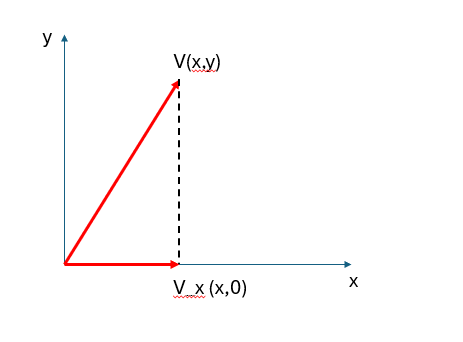
\includegraphics[scale = 1]{project1.png}\\
If we have a vector that is along the x axis
\begin{align*}
X = \left( \begin{array} {c }
              1  \\
              0  \\
            \end{array} \right)\\
\end{align*}
 The projection matrix of a vector into x line is 
\begin{align*}
P_x & = x(x^Tx)^{-1}x^T \\
     & = \left( \begin{array} {c}
              1 \\
              0 \\
            \end{array} \right)
 \left( \begin{array} { c  c } 
                   1 & 0\\
           \end{array} \right) \\
       & =  \left( \begin{array} { c  c } 
                   1 & 0  \\
                   0 & 0  \\
           \end{array} \right)
\end{align*}
Applying this projection matrix to any 2 dimensional vector $V$ gives $(V_x, 0)^T$. So it projects the vector into x line. 
Let us take another example. Imagine $V_1$ is vector if we project $V$ onto the line that has 45 degree angle with x axis. See below.

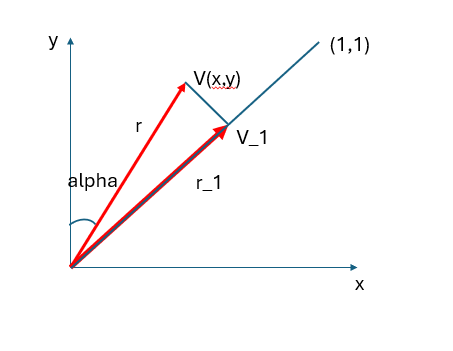
\includegraphics[scale = 1]{project2.png}\\

In order to calculate $V_1$,  we see
\begin{align*}
r_1 = r cos(\pi/4 - alpha) =r( \frac{\sqrt{2}}{2} \frac{y}{r} + \frac{\sqrt{2}}{2} \frac{x}{r}) = \frac{\sqrt 2}{2}y +\frac{\sqrt2}{2} x
\end{align*}
\begin{align*}
V_{1x}=r_1cos(\pi/4)=\frac{x+y}{2}\\
V_{1y}=r_1sin(\pi/4)=\frac{x+y}{2}\\
\end{align*}
After we understand this using geometry point of view, we can workout from algebra point of view. The vector we want to project onto is
\begin{align*}
i = \left( \begin{array} {c }
              1  \\
              1  \\
            \end{array} \right)\\
\end{align*}
The projection matrix of a vector into x line is 
\begin{align*}
P_x & = x(x^Tx)^{-1}x^T \\
     & = \left( \begin{array} {c}
              1 \\
              1 \\
            \end{array} \right)
\left( \left( \begin{array} {c c}
              1 & 1\\
            \end{array} \right) 
          \left( \begin{array} {c }
              1 \\
              1 \\
            \end{array} \right) \right)^{-1}
 \left( \begin{array} { c  c } 
                   1 & 1\\
           \end{array} \right) \\
       & =  \frac{1}{2}\left( \begin{array} { c  c } 
                   1 & 1  \\
                   1 & 1  \\
           \end{array} \right)
\end{align*}
Therefore we easily see
\begin{align*}
V_1 =  \frac{1}{2}\left( \begin{array} { c  c } 
                   1 & 1  \\
                   1 & 1  \\
           \end{array} \right) 
             \left( \begin{array} {c }
              x \\
              y \\
            \end{array} \right)
          = \left( \begin{array} {c }
              \frac{1}{2} (x+y) \\
              \frac{1}{2} (x+y) \\
            \end{array} \right)
\end{align*}
which is the same as what we get based on geometry.
 For n dimensional vector y, if our X matrix has rank of k, then the projection matrix P projects the vector y into k dimensional hyperplane. For example, if we define
\begin{align*}
i_N =   \left( \begin{array} {c }
              1 \\
              1 \\
             ...\\
              1
            \end{array} \right)
\end{align*}
The projection matrix P is
\begin{align*}
P = i \frac{1}{N}i^T
  = \frac{1}{N} \left( \begin{array} { c  c c c } 
                   1 & 1 & ... & 1 \\
                   1 & 1 & ... & 1 \\
                   ... & ... & ... & ... \\
                   1 & 1 & ... & 1 \\
           \end{array} \right) 
\end{align*}
{\bf Projection matrix into null space}\\
If $P$ is a projection matrix, the matrix $I - P$ is also a projection matrix. In linear regression model
\begin{align*}
y &= X\beta +\epsilon\\
P &= X(X^TX)^{-1}X^T\\
\hat \epsilon & = (I - P) y = (I - X(X^TX)^{-1}X^T)y\\
\end{align*}
For the above example, we define $M = I - \frac{1}{N}i i^T$, and $My$ express the mean deviations of a vector.\\
{\bf Idempotent property of projection matrix\\}
Consider the previous example that we project a vector V onto x axis, how about we do this projection twice, we would end up the same vector $V_x$. Using a little matrix algebra, it is easy to prove that for any project matrix P, we have $PP=P$.  
\subsection{Partitioned Regression and Partial Regression}
\begin{align*}
y = X \boldsymbol \beta + \epsilon = X_1 \beta_1 + X_2 \beta_2 + \epsilon
\end{align*}
The normal equation is
\begin{align*}
 \left( \begin{array} { c  c } 
                   X_1^TX_1 & X_1^TX_2  \\
                   X_2^TX_1 & X_2^TX_2   \\
           \end{array} \right)
 \left( \begin{array} { c  } 
                   \hat \beta_1   \\
                   \hat \beta_2   \\
           \end{array} \right) =
\left( \begin{array} { c  } 
                   X_1^T y   \\
                   X_2^T y   \\
           \end{array} \right)
\end{align*}
If X1 and X2 are orthogonal, namely, $X_1^T X_2=0$, then 
\begin{align*}
\boldsymbol {\hat  \beta_1} = (X_1^T X_1)^{-1} X_1^Ty\\
\boldsymbol {\hat  \beta_2} = (X_2^T X_2)^{-1} X_2^Ty
\end{align*}
\begin{align*}
\hat \beta_2 & = [X_2^T(I-X_1(X_1^TX_1)^{-1}X_1^T)X_2]^{-1}[X_2(I-X_1(X_1^TX_1)^{-1}X_1^T)y]\\
& = (X_2^T M_1 M_1X_2)^{-1}(X_2^T M_1 M_1y) \\
& = (X_2^T M_1^T M_1X_2)^{-1}(X_2^TM_1^T M_1y) \\
& = ((M_1 X_2)^T  M_1X_2)^{-1}((M_1 X_2)^T M_1y) 
\end{align*}
The above uses the property that $M_1^T=M_1$ and $M_1 M_1 = M_1$\\
The $\hat \beta_2$ is also the solution of 
\begin{align*}
 M_1 y = M_1 X_2 \beta + \epsilon
\end{align*}
where $M_1 y$ is the residual of y regressed on $X_1$ and $M_1 X_2$ is the residual of $X_2$ regressed on $X_1$.
\subsection{Variance of $\hat \beta$ and $\sigma^2$ estimation}
\begin{align*}
Var(\hat \beta)
=Var((X^TX)^{-1}X^T \epsilon)
=(X^TX)^{-1}X^T Var( \epsilon) ((X^TX)^{-1}X^T)^T\\
=\sigma^2 (X^TX)^{-1}X^T  X (X^TX)^{-1}
=\sigma^2 (X^TX)^{-1}
\end{align*}
For simple linear regression
\begin{align*}
Var(\hat \beta)
=\frac{\sigma^2}{n\Sigma x_i^2 - (\Sigma x_i)^2} \left(  \begin{array} {cc}
	          \Sigma_i x_i^2 & -\Sigma_i x_i \\
		 -\Sigma_i x_i &n\\
		\end{array}
		\right) 
\end{align*}
\begin{align*}
Var(\hat \beta_0) =\frac{\Sigma x_i^2 \sigma^2}{n\Sigma x_i^2 - (\Sigma x_i)^2} 
\end{align*}
\begin{align*}
Var(\hat \beta_1) =\frac{n \sigma^2}{n\Sigma x_i^2 - (\Sigma x_i)^2} 
\end{align*}
Try
\begin{align*}
\Sigma (x_i- \bar x)^2 = \Sigma(x_i^2 - 2 \bar x x_i+ \bar x^2)
= \Sigma_i(x_i^2 - 2 (\Sigma_j \frac{x_j}{n}) x_i + \frac{ (\Sigma_j x_j)^2} {n^2})\\
=\Sigma_ix_i^2 - \frac{2}{n} (\Sigma_i x_i)^2 + \frac{ (\Sigma_i x_i)^2} {n}
= \Sigma_i x^2_i - \frac{1}{n} (\Sigma x_i)^2
\end{align*}
So
\begin{align*}
Var(\hat \beta_0) =\frac{\Sigma x_i^2 \sigma^2}{n\Sigma (x_i- \bar x)^2 } 
\end{align*}
\begin{align*}
Var(\hat \beta_1) =\frac{n \sigma^2}{n\Sigma (x_i- \bar x)^2} = \frac{\sigma^2}{\Sigma (x_i- \bar x)^2}
\end{align*}
\begin{align*}
SSE
&=\Sigma_i (y-\hat y_i)^2 \\
& = (Y-X\beta)^T(Y-X\beta) \\
& = (Y-X(X^TX)^{-1}X^TY)^T(Y-X(XTX)-1X^TY) \\
& = (Y-PY)^T(Y-PY) \\
& = Y^T(1-P)^T(1-P)Y = Y^T(1-P)Y \\
& = (X\beta + \epsilon) ^T (1-P)(X\beta+\epsilon) \\
& = \beta^T X^T (1-P)X\beta + 2\beta^T X^T X^T(I-P)\epsilon 
   + \epsilon^T(I-H)\epsilon 
\end{align*}
\begin{align*}
E[SSE] = E[\epsilon^T(I-P)\epsilon] = E[\epsilon^T \epsilon] trace(I-H)
          = \sigma^2(n-k)\\
\end{align*}
We obtain the unbiased estimator of $\sigma^2$\\
\begin{align*}
\hat \sigma^2 = \frac{SSE}{n-k}
\end{align*}
Therefore the estimator of variance of $\beta$
\begin{align*}
\hat Var(\hat \beta_i) = \hat \sigma^2(X^TX)^{-1}_{ii}
\end{align*}
and the stanard error of $\beta_i$ is
\begin{align*}
SE(\hat \beta_i) = \sqrt{ \hat \sigma^2(X^TX)^{-1}_{ii}}
\end{align*}
\section{Properties of Least Square Estimators}
\subsection{Unbiasness}
When we have a estimator, we need to ask ourselves two questions, 1)how accurate is our estimator, can the estimator give us true value of $\beta$, 2) Does it converge to the real value with reasonable speed as sample size increases? The metric we use to evaluate accuracy is unbiasness, and the metric we measure the convergence speed is the efficiency.\\ 
{\bf Unbiased}\\
\begin{align*}
\hat \beta & = (X^T X)^{-1}X^TY\\
               & = (X^T X)^{-1}X^T(X \beta + \epsilon)\\
               & = (X^T X)^{-1}X^T X \beta   + (X^T X)^{-1}X^T \epsilon\\
               & = \beta +  (X^T X)^{-1}X^T \epsilon\\
\end{align*}
Then the expectation of $\hat \beta$ condition on X is
\begin{align*}
E[{\hat \beta|X}] = \beta + (X^TX)^{-1} X^T E(\epsilon|X)\\
\end{align*}
The last term is zero by assuption of linear regression. So 
\begin{align*}
E[\hat \beta] = \beta
\end{align*}
The expectation of the estimator is the same as true value, this is called {\bf unbiased}. \\
{\bf Bias due to omission of relevant variables}\\
Suppose we have a model
\begin{align*}
y = X_1 \beta_1 + X_2 \beta_2 + \epsilon
\end{align*}
If we regression y on $X_1$ only, our estimator is
\begin{align*}
\hat \beta_1 = (X_1^T X_1)^{-1} X_1^T y = \beta_1 + (X_1^TX_1)^{-1}X_1^TX_2\beta_2 + (X_1^TX_1)^{-1}X_1^T\epsilon
\end{align*}
On the second term, we see unless 1)$X_1$ and $X_2$ are orthogonal, or 2)$\beta_2$ =0,  $\beta_1$ is biased.\\
\subsection{Consistency}
We know
\begin{align*}
\hat \beta = \beta + (X^TX)^{-1}X^T\epsilon
\end{align*}
\begin{align*}
X^TX & = \Sigma_{i=1}^N
 \left( \begin{array} { c  c  c c } 
                   x_{1i}^Tx_{i1} & x_{1i}^Tx_{i2} & ... & x^T_{1i}x_{ik}   \\
                   ... & ... & ... & \\
                   x_{ki}^Tx_{i1} & x_{ki}^Tx_{k2} & ... & x^T_{ki}x_{ik}   \\
           \end{array} \right) \\
    & =  \Sigma_{i=1}^N
 \left( \begin{array} { c  c  c c } 
                   x_{i1}x_{i1} & x_{i1}x_{i2} & ... & x_{i1}x_{ik}   \\
                   ... & ... & ... & \\
                   x_{ik}x_{i1} & x_{ik}x_{k2} & ... & x_{ik}x_{ik}   \\
           \end{array} \right) \\
      &  =  \Sigma_{i=1}^N
 \left( \begin{array} { c  } 
                   x_{i1}    \\
                   ...  \\
                   x_{ik}    \\
           \end{array} \right)
 \left( \begin{array} { c c c c } 
                   x_{i1}  & ... &  ... x_{ik}\\ 
           \end{array} \right) \\
     & = \Sigma_{i=1}^N X_i X_i^T
\end{align*}
\begin{align*}
\hat \beta &= \beta + ({X^TX})^{-1} {X^T \epsilon} \\
               &= \beta + ( \Sigma_{i=1}^N X_i X_i^T)^{-1} X^T \epsilon \\
               &= \beta + ( \Sigma_{i=1}^N  \frac{1}{N}{X_i^TX_i})^{-1}(\frac{X^T \epsilon}{n})
\end{align*}
If $X_i$s are iid, then by law of large numbers
\begin{align*}
\Sigma_{i=1}  \frac{1}{n}{X_i^TX_i} 
\end{align*}
converges to Q in probability.\\
There are certain conditions in which the estimators become inconsitent.\\
1) X is not full rank, or X has multicollinearity
2) $cov[X, \epsilon] \neq 0$
\subsection{Multicollinearity}
Suppose we have a regression model that contains two parameters
\begin{align*}
y = \beta_0 + X_1\beta_1 + X_2 \beta_2
\end{align*}
From above, we know variance of ${\bf \hat \beta}$ is
\begin{align*}
Var(\hat \beta) = \frac{\sigma^2}{(X^TX)^{-1}}
\end{align*}
When X only contains 2 variables, $X=(X_1, X_2)$
\begin{align*}
Var(\hat \beta_1) = \sigma^2 \frac{S_{22}}{S_{11}S_{22}-S_{12}^2} = \frac{1}{S_{11}(1-\frac{S^2_{12}}{S_{11}S_{22}})}= \frac{1}{S_{11}(1-r_{12}^2)} \\
Var(\hat \beta_2) = \sigma^2 \frac{S_{11}}{S_{11}S_{22}-S_{12}^2} = \frac{1}{S_{22}(1-\frac{S^2_{12}}{S_{11}S_{22}})}= \frac{1}{S_{22}(1-r_{12}^2)} \\
\end{align*}
Where
\begin{align*}
S_{11} & =\Sigma(x_{1i}-\hat x_1)^2\\
S_{22} & =\Sigma(x_{2i}-\hat x_2)^2\\
S_{12} & =\Sigma(x_{1i}-\hat x_1)(x_{2i}-\hat x_2)\\
r_{12} & = \frac{S_{12}}{\sqrt{S_{11}S_{22}}}\\
\end{align*}
$r_{12}$ is the correlation coefficient. In extreme case, when $X_1$ and $X_2$ are perfectly correlated, the variance becomes infinite.\\
\subsection{Model Testing}
{\bf Lagrange Multiplie(LM) test}\\
Suppose we have two models, one is restriced, the other is unrestricted:
Restricted(R): $y = X_1 \beta_1 + \epsilon$\\
Unrestricted (U): $y = X_1 \beta_1 + X_2 \beta_2 + \epsilon$\\
Given the unrestriced model, the likehood function is 
\begin{align*}
L(\beta_1, \beta_2, \sigma^2) = \frac{1}{(2\pi \sigma^2)^{n/2}}exp(-\frac{1}{2\sigma^2}(y-X_1\beta_1-X_2\beta_2)^T(y-X_1\beta_1-X_2\beta_2))
\end{align*}
\begin{align*}
S_2 = \frac{\partial L}{\partial \beta_2} =\frac{1}{\sigma^2}X_2^T(y - X_1\beta_1-X_2\beta_2)
\end{align*}
When $\beta=0$, define
\begin{align*}
M_1 = I - X_1(X^T_1X_1)^{-1}X^T_1
\end{align*}
and $M_1X_1=0$.
\begin{align*}
S_2 =\frac{1}{\sigma^2}X_2^TM_1y = \frac{1}{\sigma^2}X_2^TM_1(X_1 \beta_1 + \epsilon) = \frac{1}{\sigma^2}X_2^TM_1 \epsilon
\end{align*}
The last equal sign uses the fact $M_1X_1 = 0$.
\begin{align*}
 Var(X_2^TM_1y) & = Var(X_2^TM_1 \epsilon) \\
             & =  X_2^TM_1Var(\epsilon)(X_2^TM_1)^T \\
             & =  X_2^TM_1 M_1^T X_2Var(\epsilon) = \sigma^2  X_2^TM_1X_2 \\
\end{align*}
So $X_2^TM_1\epsilon$ follows normal distribution with mean 0 and variance $\sigma^2X_2^TM_1X_2$. Define
\begin{align*}
Z=\frac{X_2^TM_1\epsilon}{\sqrt{\sigma^2X_2^TM_1X_2}}
\end{align*}
then Z follows standard normal distribution. The {\bf Lagrange Multiplier (LM) test} is defined
\begin{align*}
LM =  Z^2  = \frac{(X_2^TM_1\epsilon)^2}{\sigma^2X_2^TM_1X_2} 
\end{align*}
which follows $\chi^2$ distribution with degree of freedom 1.\\
{\bf F test}\\
We define
\begin{align*}
SSE_U = ||y -X_1\hat\beta_1 - X_2\hat\beta_2||^2\\
SSE_R = ||y -X_1\hat\beta_1 ||^2
\end{align*}
F test is defined as
\begin{align*}
F = \frac{\frac{Extra \hspace{1mm} expalined \hspace{1mm} variation}{Degree \hspace{1mm} of \hspace{1mm} Freedom}}{\frac{Remaining \hspace{1mm}  unexplained \hspace{1mm} variation}{Degree \hspace{1mm} of \hspace{1mm} Freedom}} = \frac{SSE_R - SSE_U}{\frac{SSE_U}{n-1}}
\end{align*}
Let $X=(X_1, X_2)$, and we define two projection matrices
\begin{align*}
P_U = X(X^TX)^{-1}X^T\\
P_R = X_1(X_1^TX_1)^{-1}X_1^T
\end{align*}
\begin{align*}
SSE_R-SSE_U=y^T(I-P_R)y-y^T(I-P_U)y = y^T(P_U-P_R)y
\end{align*}
recall
\begin{align*}
\hat \beta_2 = (X_2^T M_1 X_2)^{-1}X_2^TM_1 y
\end{align*}
So 
\begin{align*}
P_U-P_R = X_2\beta =X_2(X_2^TM_1X_2)^{-1}X_2^TM_1y\\
SSR_R-SSR_U = (X_2^TM_1y)^T(X_2^TM_1X_2)^{-1}X_2^TM_1y
\end{align*}
\begin{align*}
F = \frac{SSR_R - SSR_U}{\frac{SSR_U}{n-k}} = \frac{(X_2M_1y)^T(X_2^TM_1y)}{\hat \sigma^2 (X_2^TM_1X_2)} =LM
\end{align*}
We see that F test and LM test are equivalent.
\end{document}